\section{Cenário de Testes}
\label{sec:cenario}

Dentro do âmbito das DTNs, é possível dissertar acerca de uma imensa quantidade de cenários possíveis para teste. Tendo em isso em vista, decidiu-se, neste trabalho, basear-se no cenário de testes definido em \cite{denis_artigo}. Além disso, foram considerados os dois estados da técnica desenvolvida: Desligada e Ligada contabilizando o consumo de GPS. Contabilizar o consumo GPS possibilita uma análise aprofundada do consumo adicional gerado pela técnica devido ao uso desses dispositivos.

O mapa da Figura \ref{mapa_tecnica} foi utilizado como base para os testes realizados e possui uma dimensão de 4500 por 3500 metros. O mesmo é baseado na cidade Helsínquia, a capital da Finlândia. A Figura \ref{mapa_helsinquia} apresenta uma sobreposição do mapa do ambiente simulado com o da cidade escolhida, permitindo perceber grande similaridade entre eles. Este mesmo mapa foi utilizado por \cite{denis_artigo}.

\begin{figure}[htp!]
\centering
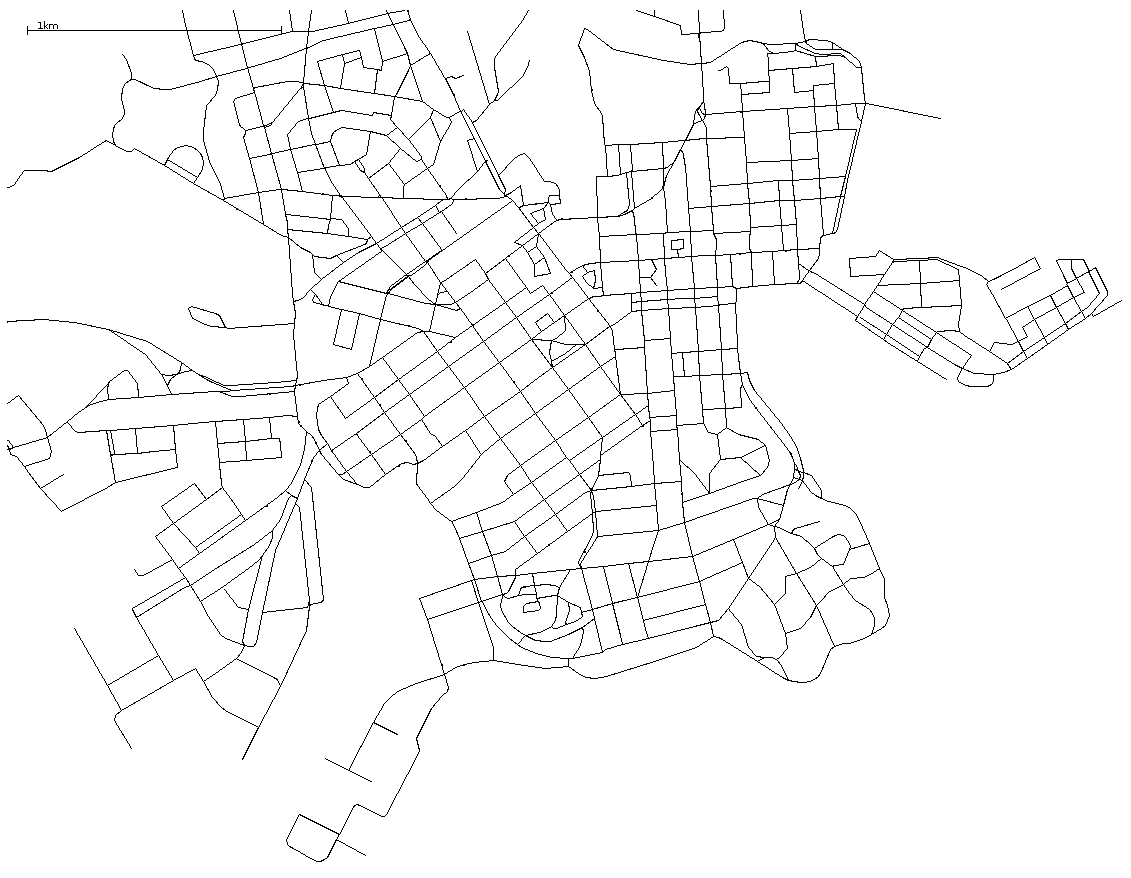
\includegraphics[width=0.9\textwidth]{figuras/cap_5/mapa.png}
\caption{Mapa utilizado nos cenários de teste \cite{keranen2009one}.}
\label{mapa_tecnica}
\end{figure}

\begin{figure}[htp!]
\centering
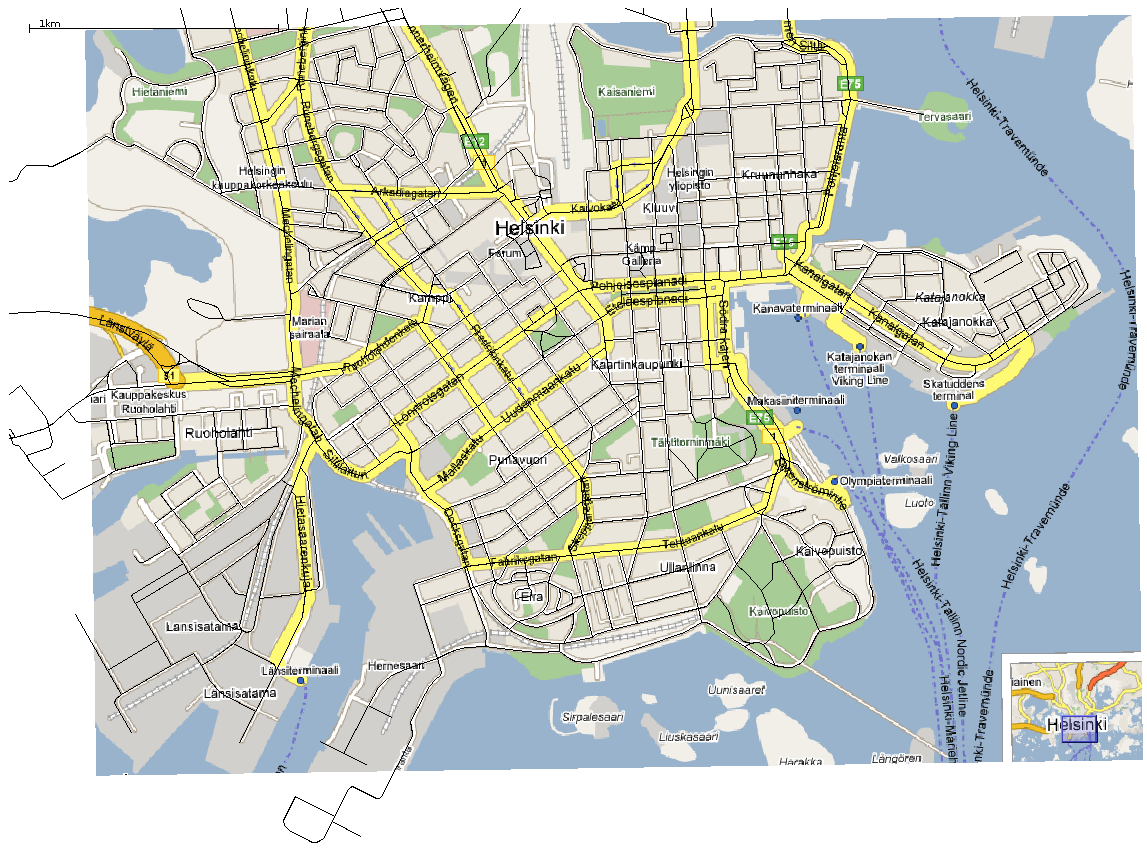
\includegraphics[width=0.9\textwidth]{figuras/cap_5/mapa_helsinquia.png}
\caption{Mapa da cidade Helsínquia \cite{keranen2009one}.}
\label{mapa_helsinquia}
\end{figure}

Foram definidas regiões quadradas com 500 metros de lado, totalizando assim um conjunto de 63 regiões. Este valor foi escolhido devido a multiplicidade com o tamanho do mapa base e por não gerar uma quantidade exorbitante de regiões a serem mapeadas. Quando objetivada uma mais análise aprofundada, este parâmetro é passível de ser verificado quanto a procura de um tamanho ideal que se adeque a limitações de memória que os dispositivos utilizados possuem e características relacionadas ao comportamento da DTN onde a técnica será utilizada.

A DTN proposta é constituída por 51 nós divididos em seis grupos. Dois deles, \emph{p} e \emph{w}, com 15 elementos cada, representam grupos de pedestres. Existe um grupo \emph{c} de 15 nós representando carros e, outros três grupos \emph{th}, \emph{tr} e \emph{tu}, com dois elementos cada, representando os bondes da cidade de Helsínquia. 

Os grupos pedestres se locomovem respeitando o modelo de movimento Shortest Path Map-Based Movement, onde os nós sempre se movimentam pelos caminhos disponíveis no mapa escolhendo pontos aleatórios e seguindo até eles pela rota mais curta partindo da sua posição atual. A velocidade com que as pessoas se movimentam pode variar entre 1,8 a 5,5 Km/h. Os carros no cenário desenvolvido utilizam o mesmo modelo de movimento dos pedestres, todavia são forçados se locomover apenas pelas ruas e desenvolvem velocidades entre 10 e 50 Km/h.

Os grupos de bondes utilizam o modelo de movimento Routed Map-Based Moviment. Neste modelo cada grupo de nós sempre se locomove por uma rota distinta dos demais. Por se tratar de bondes, os mesmos realizam paradas em locais pré-determinados por períodos de dez a trinta segundos. A velocidade desses nós varia de 25 e 36 km/h. 

A Tabela \ref{grupos_nos} apresenta de forma sucinta os dados dos grupos de nós definidos para o cenário de simulação.

Devido a uma limitação do simulador The ONE, não é possível que pessoas entrem e saiam dos carros e bondes. Para contornar isso, assumiu-se que os condutores de cada um dos veículos portam o mesmo tipo dispositivo utilizado pelos pedestres. Por sua vez, os dispositivos utilizados por todos os indivíduos da rede constem em \emph{smartphones} com baterias de 4800mW e interfaces \emph{bluetooth} para a troca de mensagens. As interfaces \emph{bluetooth} possuem um alcance de 10 metros e velocidade de transmissão de 2Mb/s. Além disso, os aparelhos possuem uma capacidade de armazenamento de 5MB.

\begin{table}
\centering
\caption{Definição dos grupos de nós.}
\label{grupos_nos}
\begin{tabular}{|c|c|c|c|c|}
\hline
Nome          & Tipo      & Velocidade     & Quantidade & Modelo de Movimento               \\ \hline
p             & Pedestres & 1,8 a 5,5 Km/h & 15         & ShortestPath  Map-Based \\ \hline
c             & Carros    & 10 a 50 Km/h   & 15         & ShortestPath  Map-Based \\ \hline
w             & Pedestres & 1,8 a 5,5 Km/h & 15         & ShortestPath  Map-Based  \\ \hline
th            & Bonde     & 25 a 36 Km/h   & 2          & Routed Map-Based         \\ \hline
tr            & Bonde     & 25 a 36 Km/h   & 2          & Routed Map-Based         \\ \hline
tu            & Bonde     & 25 a 36 Km/h   & 2          & Routed Map-Based         \\ \hline
\end{tabular}
\end{table}

Os parâmetros de energia, essenciais neste trabalho, seguem também o mesmo modelo de consumo proposto por \cite{denis_artigo} e são apresentados na Tabela \ref{consumo_denis_artigo}. Os \emph{smartphones} iniciam com a bateria totalmente carregada e ela vai descarregando a medida em que fazem operações de busca, envio e recepção de mensagens. Adicionalmente, é considerado o consumo dos dispositivos GPS explanado na Subseção \ref{subsec:consumo_gps}, ou seja, 154,6mW a cada consulta realizada. 

\begin{table}
\centering
\caption{Parâmetros de energia utilizados.}
\label{consumo_denis_artigo}
\begin{tabular}{|c|c|}
\hline
Parâmetros                   & Definições    \\ \hline
Capacidade da bateria        & 4800mW        \\ \hline
Consumo da Busca             & 0.92mW/busca \\ \hline
Consumo enviando mensagem    & 0.08mW/s\\ \hline
Consumo recebendo mensagem   & 0.08mW/s\\ \hline
Consumo do dispositivo GPS   & 0.1546mW/consulta \\ \hline
\end{tabular}
\end{table}

Quanto aos protocolos de encaminhamento, foram considerados os protocolos \emph{Epidemic Routing}, \emph{Prophet} e \emph{Spray-and-Wait}, detalhados na Subseção \ref{subsec:encaminhamento_mensagens}. 

Além disso, é inerente, na análise de desempenho da técnica, levar em consideração a procura por um intervalo de busca ótimo. No entanto, optou-se neste trabalho por estudá-lo em apenas duas combinações próximas ao período de 32 segundos apresentado por \cite{denis_artigo}. A primeira, com 8, 32 e 56 segundos, com variação de 16 segundos para mais e para menos; a segunda, com 8, 32 e 32 segundos, com apenas uma variação de 16 segundos para menos. Os valores se referem à ordem dos intervalos de cada combinação, sendo o mínimo, padrão e máximo, respectivamente.

Os tempos de simulação consistem em períodos de 10 e 30 dias e são realizadas análises quanto a recarga periódica completa das baterias.